\begin{figure}[tp]
	\centering
	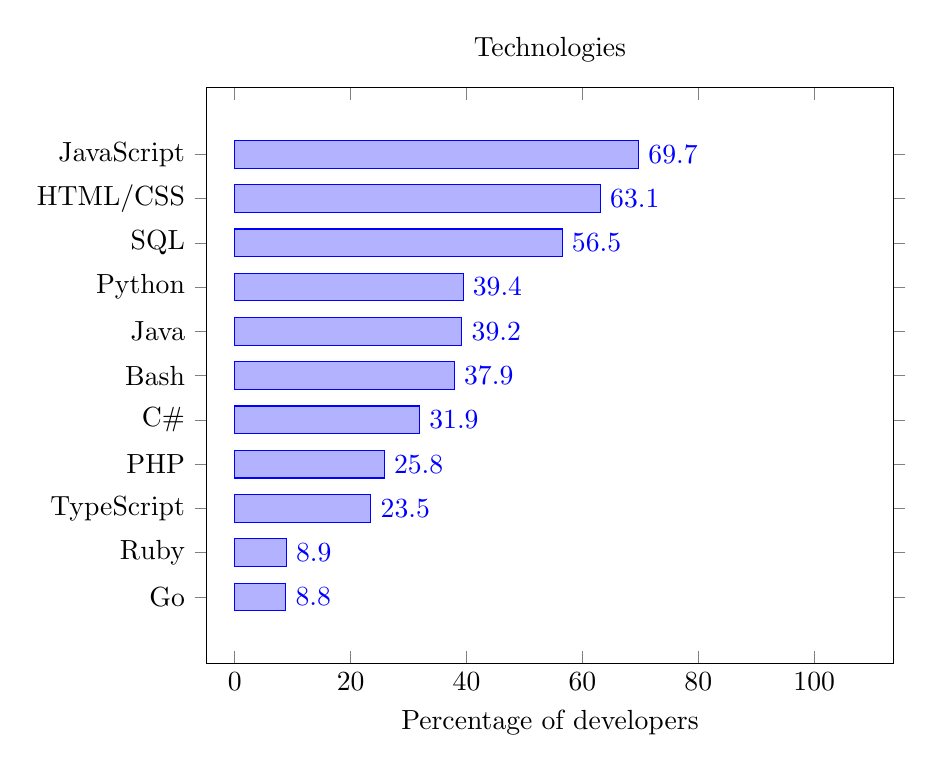
\begin{tikzpicture}
		\begin{axis}[
			xbar,
			title=Technologies,
			width=0.85\textwidth,
			xbar=0pt,
			xmax=100,
			enlargelimits=0.15,
			legend style={at={(0.5,-0.2)}, anchor=south,legend columns=-1},
			xlabel=Percentage of developers,
			symbolic y coords={
				Go,
				Ruby,
				TypeScript,
				PHP,
				C\#,
				Bash,
				Java,
				Python,
				SQL,
				HTML/CSS,
				JavaScript,
			},
			ytick=data,
			nodes near coords, 
			y tick label style={anchor=east},
			every axis plot/.append style={
				bar shift=0pt,
				fill
			  }
		]
		\addplot coordinates {
			(69.7,JavaScript)
			(63.1,HTML/CSS)
			(56.5,SQL)
			(39.4,Python)
			(39.2,Java)
			(37.9,Bash)
			(31.9,C\#)
			(25.8,PHP)
			(23.5,TypeScript)
			(8.9,Ruby)
			(8.8,Go)
		};
		\end{axis}
	\end{tikzpicture}
	%
	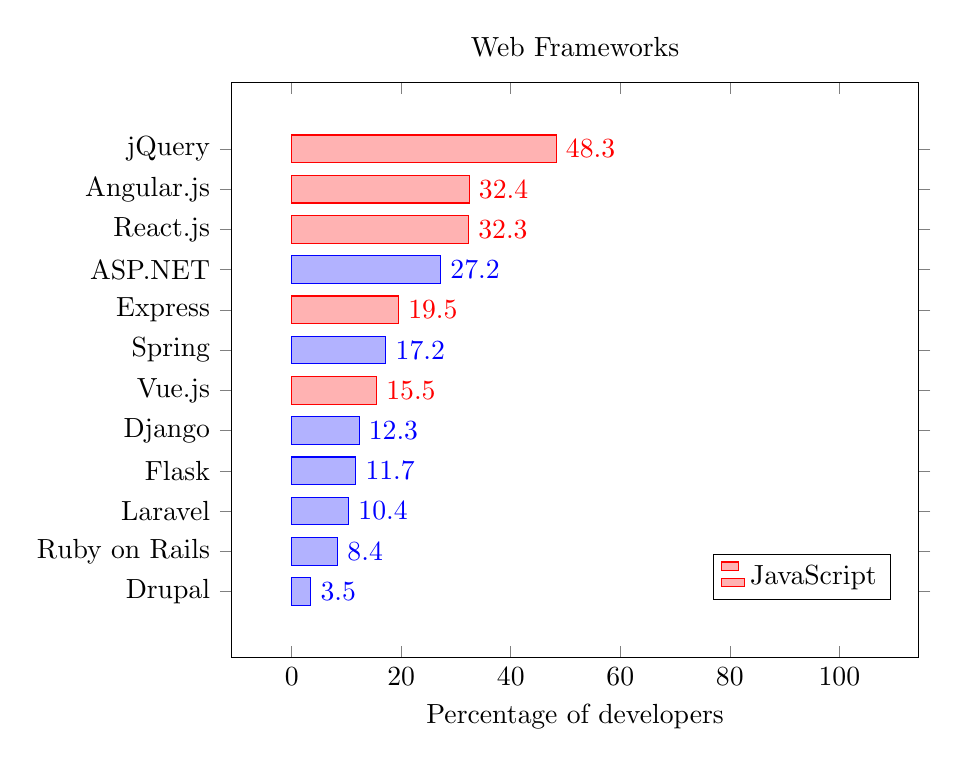
\begin{tikzpicture}
		\begin{axis}[
			xbar,
			title=Web Frameworks,
			width=0.85\textwidth,
			xbar=0pt,
			xmax=100,
			enlargelimits=0.15,
			legend style={at={(0.7,0.1)}, anchor=south west,legend columns=-1},
			xlabel=Percentage of developers,
			yticklabels={
				jQuery,
				Angular.js,
				React.js,
				ASP.NET,
				Express,
				Spring,
				Vue.js,
				Django,
				Flask,
				Laravel,
				Ruby on Rails,
				Drupal,
			},
			ytick={12, 11, ..., 1},
			nodes near coords, 
			y tick label style={anchor=east},
			every axis plot/.append style={
				bar shift=0pt,
				fill
			  }
		]

		\addplot coordinates {
			(27.2,9)
			(17.2,7)
			(12.3,5)
			(11.7,4)
			(10.4,3)
			(8.4,2)
			(3.5,1)
		};

		\addplot coordinates {
			(48.3,12)
			(32.4,11)
			(32.3,10)
			(19.5,8)
			(15.5,6)
		};

		\legend{,JavaScript}
		\end{axis}
	\end{tikzpicture}
	\caption[Conditional operators]{\textbf{Most Popular Technologies \& Frameworks 2019} - According to Stackoverflow's Developer Survey, JavaScript is the most commonly used programming language for 2019. 5 out of 12 of the most popular Web Frameworks are written in JavaScript.
	\label{fig:background-survey-programming-languages}
	}
\end{figure}